\lab{Application}{Image Processing and Filters}{Image Filters}

\objective{Explore Image Filters. In particular, we will explore the Sobel Filter, which uses numerical derivatives to find edges in images.}

One of the primary tools in image processing is the use of filters to identify important information in images. In this section we will implement our own filters and explore applications.

One of the easiest filters to implement is matrix based. In this implementation, the filter that we select is a matrix, which represents how much we want certain pixels to contribute to the output image. Suppose that we choose our filter to be:

\[
A = \begin{pmatrix}
a_{11}&a_{12}&a_{13}\\
a_{21}&a_{22}&a_{23}\\
a_{31}&a_{32}&a_{33}
\end{pmatrix}
\]

We will call our input image (Matrix) B and our ouput image (Matrix) C. This type of filter works according to the following formula:
\[
C_{ij} = \sum_{k=-1}^1 \sum_{m=-1}^1 a_{km}*B_{(i+k,j+m)}
\]

Essentially this computes each pixel of the output image as the weighted sum of the surrounding pixels in the input image. The technical term for this type of operation is a convolution.

\begin{problem}
Write a function that will take as input an arbitrary filter matrix and image and output the filtered image. Note that for these filters to be meaningful they will need to be odd by odd (there are ways to handle even size filters, but we won't handle them here). Have MATLAB return an error message if the filter is not of appropriate size. You may choose how to handle the edges of the image, but we suggest simply copying the edge pixels out.

You can test your function by loading a sample image using the command imread, with a file chosen from the MATLAB demos (pick one from {\tt help imdemos}). You can then apply the identity filter, which is any n by n matrix where n is odd and the only non-zero entry is a one in the very center of the matrix. Use the command {\tt imshow} on both the input and output image. They should be the same.
\end{problem}

So what can we do with these filters? We will show an example of how to apply a gaussian blur using this type of filter. To begin, load the following picture:

\begin{verbatim}
K = imread('cameraman.tif');
imshow(K);
\end{verbatim}

{\tt imshow} should display an image like this one:

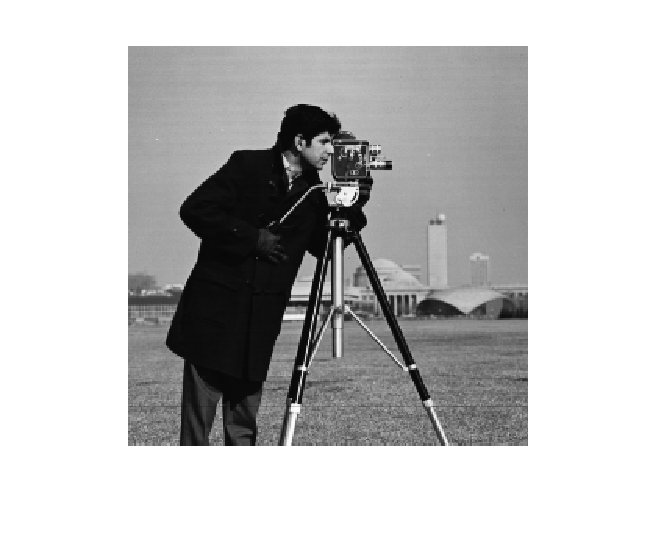
\includegraphics{./Figures/cameramanClean.pdf}

Now that you have a simple filter function try the following filter on this image:

\[
A = \frac{1}{159}\begin{pmatrix}
2&4&5&4&2\\
4&9&12&9&4\\
5&12&15&12&5\\
2&4&5&4&2\\
4&9&12&9&4
\end{pmatrix}
\]

You should get an output that looks something like this:

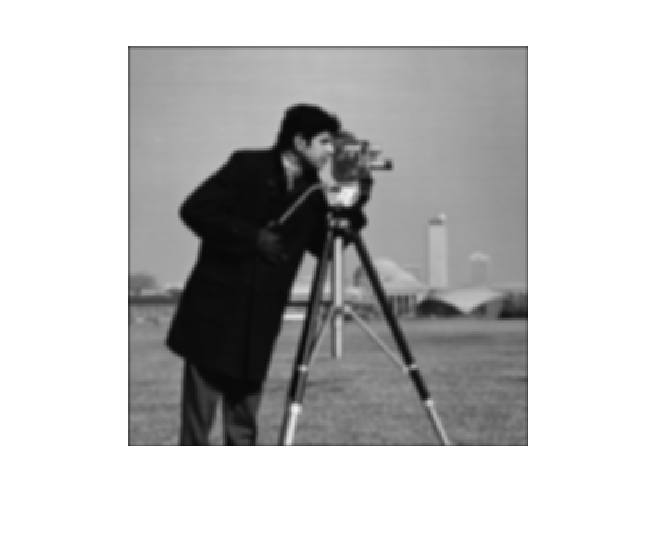
\includegraphics{./Figures/cameramanBlur.pdf}

You can see that the filter blurred the image. This can be very important in trying to wash out images that are ``noisy.''

\begin{problem}

The Sobel Filter is a filter used in edge detection. It works by using a numerical approximation of the gradient to find edges in the image. The filter to find the gradient in the y direction is:

\[
A = \frac{1}{8}\begin{pmatrix}
-1&-2&-1\\
0&0&0\\
1&2&1
\end{pmatrix}
\]

The gradient in the x direction is simply the transpose of that matrix.

Write a simple function that finds the edges of an image using the sobel filter. You will probably need to preprocess the image using the function {\tt im2single}. You will then find the magnitude of the gradient by combining the x and y gradient matrices (what is the correct way to do this?). Lastly, you will need to look for places where the magnitude of the gradient is large enough (the location of edges) by looking at values over a threshold (which you'll also need to find). We found four times the mean of the output image to be pretty good. On the camerman example we had the following output:
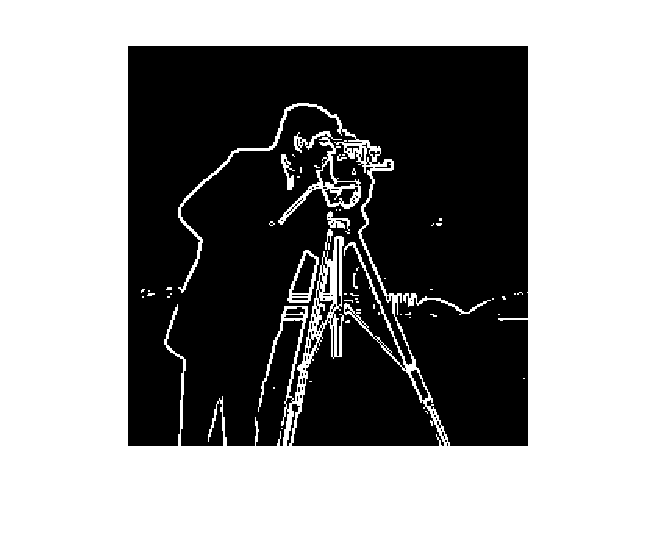
\includegraphics{./Figures/edges.pdf}
\end{problem}
